% SPDX-License-Identifier: AGPL-3.0-or-later
% The picture in 10-scaled-figure.tex: lualatex soliton.tex makes soliton.pdf.
\documentclass[border=2pt]{standalone}
\usepackage{pgfplots}
\pgfplotsset{compat=1.18}
\begin{document}
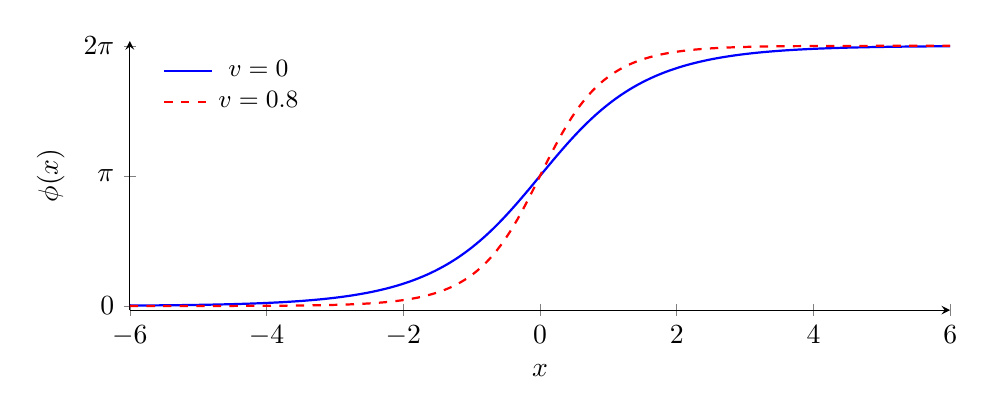
\begin{tikzpicture}
\begin{axis}[width=12cm, height=5cm, xmin=-6, xmax=6, ymin=-0.1, ymax=6.4,
  xlabel={$x$}, ylabel={$\phi(x)$}, axis lines=left, samples=200,
  ytick={0,3.14159,6.28318}, yticklabels={$0$,$\pi$,$2\pi$},
  legend pos=north west, legend style={draw=none, fill=none, font=\small}]
\addplot[thick, blue, domain=-6:6] {4*rad(atan(exp(x)))};
\addlegendentry{$v=0$}
\addplot[thick, red, dashed, domain=-6:6] {4*rad(atan(exp(x/sqrt(1-0.8^2))))};
\addlegendentry{$v=0.8$}
\end{axis}
\end{tikzpicture}
\end{document}
